\section{Samenvattende Schema's}
\subsection{Zoekmethodes}
\label{app:schemaSearch}
\begin{figure}[H]
\centering
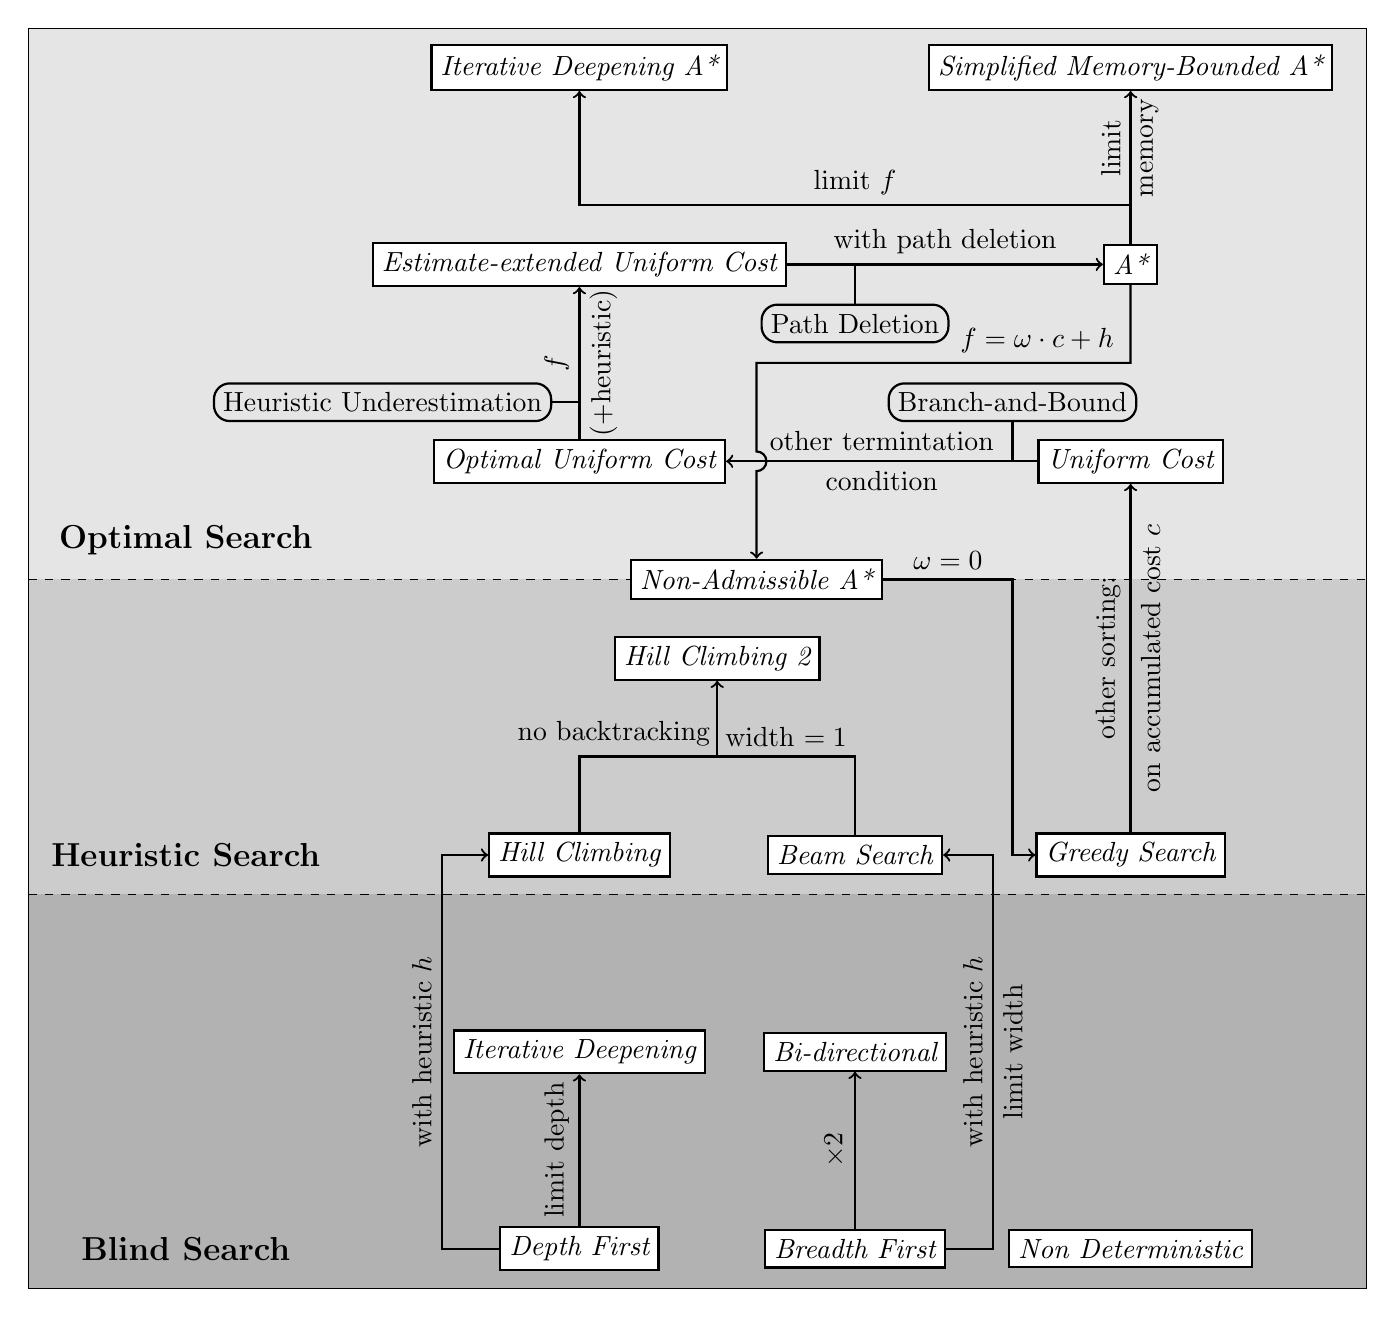
\begin{tikzpicture}[algor/.style={draw=black,thick,fill=white,font=\itshape},principle/.style={shape=rectangle,rounded corners=2mm,draw=black,thick,fill=black!10},hasinspired/.style={thick,->},hasinspirednoarrow/.style={thick},withprinciple/.style={thick,}]
\fill[black!30] (-2,-0.5) rectangle (15,4.5);
\fill[black!20] (-2,4.5) rectangle (15,8.5);
\fill[black!10] (-2,8.5) rectangle (15,15.5);
\draw (-2,-0.5) rectangle (15,15.5);
\draw[dashed] (-2,4.5) -- (15,4.5);
\draw[dashed] (-2,8.5) -- (15,8.5);
\draw[double] (0,0) node{\bf \large Blind Search};
\draw (0,5) node{\bf \large Heuristic Search};
\draw (0,9) node{\bf \large Optimal Search};
\node[algor] (df) at (5,0) {Depth First};
\node[algor] (bf) at (8.5,0) {Breadth First};
\node[algor] (nd) at (12,0) {Non Deterministic};
\node[algor] (id) at (5,2.5) {Iterative Deepening};
\node[algor] (bd) at (8.5,2.5) {Bi-directional};
\node[algor] (hc) at (5,5) {Hill Climbing};
\node[algor] (bs) at (8.5,5) {Beam Search};
\node[algor] (hc2) at (6.75,7.5) {Hill Climbing 2};
\node[algor] (gs) at (12,5) {Greedy Search};
\node[algor] (uc) at (12,10) {Uniform Cost};
\node[algor] (ouc) at (5,10) {Optimal Uniform Cost};
\node[algor] (euc) at (5,12.5) {Estimate-extended Uniform Cost};
\node[algor] (as) at (12,12.5) {A*};
\node[algor] (idas) at (5,15) {Iterative Deepening A*};
\node[algor] (smbas) at (12,15) {Simplified Memory-Bounded A*};
\node[algor] (naas) at (7.25,8.5) {Non-Admissible A*};
\node[principle] (bab) at (10.5,10.75) {Branch-and-Bound};
\node[principle] (hu) at (2.5,10.75) {Heuristic Underestimation};
\node[principle] (pd) at (8.5,11.75) {Path Deletion};
\draw[hasinspired] (df) to node[midway,above,rotate=90]{limit depth} (id);
\draw[hasinspired] (bf) to node[midway,above,rotate=90]{$\times2$} (bd);
\draw[hasinspired] (df) -- (3.25,0) to node[midway,above,rotate=90]{with heuristic $h$} (3.25,5) -- (hc);
\draw[hasinspired] (bf) -- (10.25,0) to node[midway,above,rotate=90]{with heuristic $h$} node[midway,below,rotate=90]{limit width} (10.25,5) -- (bs);
\draw[hasinspired] (hc)  -- (5,6.25) to node[near start,above]{no backtracking}  (6.75,6.25) -- (hc2);
\draw[hasinspirednoarrow] (bs) -- (8.5,6.25) to node[midway,above]{width $=1$} (6.75,6.25);
\draw[hasinspired] (gs) to node[midway,above,rotate=90]{other sorting:} node[midway,below,rotate=90]{on accumulated cost $c$} (uc);
\draw[hasinspired] (uc) to node[midway,above]{other termintation} node[midway,below]{condition} (ouc);
\draw[withprinciple] (bab) -- (10.5,10);
\draw[hasinspired] (ouc) to node[midway,above,rotate=90]{$f$} node[midway,below,rotate=90]{(+heuristic)} (euc);
\draw[withprinciple] (hu) -- (5,10.75);
\draw[hasinspired] (euc) to node[midway,above]{with path deletion} (as);
\draw[withprinciple] (pd) -- (8.5,12.5);
\draw[hasinspired] (as) -- (12,13.25) to node[midway,above]{limit $f$} (5,13.25) -- (idas);
\draw[hasinspired] (12,13.25) to node[midway,above,rotate=90]{limit} node[midway,below,rotate=90]{memory} (smbas);
\draw[hasinspired] (naas)  to node[midway,above]{$\omega=0$} (10.5,8.5) |- (gs.west);
\draw[hasinspired] (as) -- (12,11.25) to node[near start,above]{$f=\omega\cdot c+h$} (7.25,11.25) -- (7.25,10.125) arc (90:-90:.125) -- (naas);
\end{tikzpicture}
\caption{Samenvattend schema van Zoekmethodes}
\end{figure}
\subsection{Constraint Processing}
\begin{figure}[H]
\centering
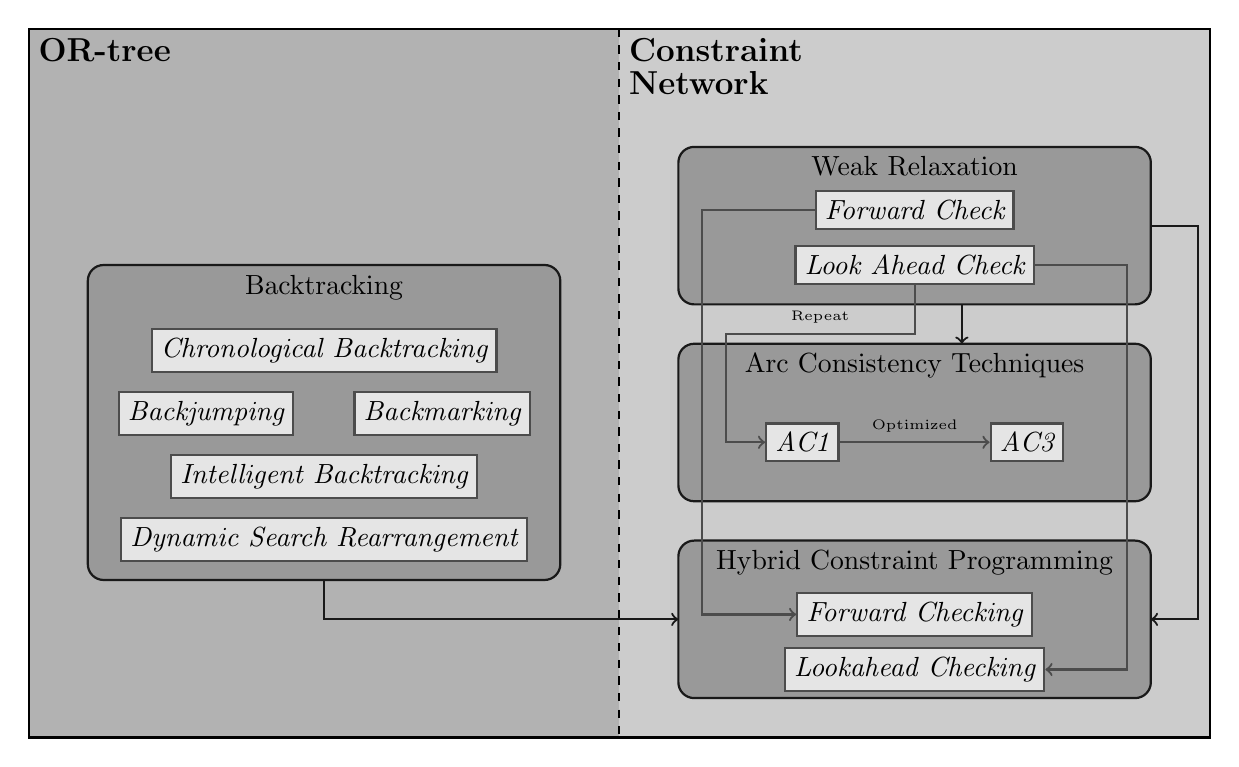
\begin{tikzpicture}[taal/.style={anchor=north west,text width=90pt},conceptgroup/.style={draw=black!90,fill=black!40, rounded corners=2mm, thick,minimum width=60mm,minimum height=20mm},hasinfluence/.style={black!90,thick,->},algor/.style={draw=black!70,thick,fill=black!10,font=\itshape},algorinfluence/.style={black!70,thick,->}]
\def\rectW{15};
\def\rectH{10};
\def\trapa{0};
\def\trapaCax{-0.25*\rectW+0.5*\trapa}
\def\trapaCay{-0.6*\rectH}
\def\trapaCaw{6}
\def\trapaCah{4}

\def\trapbCax{0.25*\rectW+0.5*\trapa}
\def\trapbCay{-0.35*\rectH}
\def\trapbCaw{6}
\def\trapbCah{2}
\def\trapbCbx{0.25*\rectW+0.5*\trapa}
\def\trapbCby{-0.6*\rectH}
\def\trapbCbw{6}
\def\trapbCbh{2}
\def\trapbCcx{0.25*\rectW+0.5*\trapa}
\def\trapbCcy{-0.85*\rectH}
\def\trapbCcw{6}
\def\trapbCch{2}

\fill[black!30] (-0.5*\rectW,-1) rectangle (\trapa,-\rectH);
\fill[black!20] (\trapa,-1) rectangle (0.5*\rectW,-\rectH);
\draw[thick] (-0.5*\rectW,-1) rectangle (0.5*\rectW,-\rectH);
\draw[thick,dashed] (\trapa,-1) -- (\trapa,-\rectH);

\node[taal] (trapaL) at (-0.5*\rectW,-1) {\bf \large OR-tree};
\draw[conceptgroup] (\trapaCax-0.5*\trapaCaw,\trapaCay-0.5*\trapaCah) rectangle (\trapaCax+0.5*\trapaCaw,\trapaCay+0.5*\trapaCah);
\node[anchor=north] (trapaG1) at (\trapaCax,\trapaCay+0.5*\trapaCah) {Backtracking};
\node[algor,anchor=north] (trapaG1A1) at (\trapaCax,\trapaCay+0.3*\trapaCah) {Chronological Backtracking};
\node[algor,anchor=north] (trapaG1A2) at (\trapaCax-0.25*\trapaCaw,\trapaCay+0.1*\trapaCah) {Backjumping};
\node[algor,anchor=north] (trapaG1A3) at (\trapaCax+0.25*\trapaCaw,\trapaCay+0.1*\trapaCah) {Backmarking};
\node[algor,anchor=north] (trapaG1A4) at (\trapaCax,\trapaCay-0.1*\trapaCah) {Intelligent Backtracking};
\node[algor,anchor=north] (trapaG1A5) at (\trapaCax,\trapaCay-0.3*\trapaCah) {Dynamic Search Rearrangement};

\node[taal] (trapbL) at (\trapa,-1) {\bf \large Constraint Network};
\draw[conceptgroup] (\trapbCax-0.5*\trapbCaw,\trapbCay-0.5*\trapbCah) rectangle (\trapbCax+0.5*\trapbCaw,\trapbCay+0.5*\trapbCah);
\node[anchor=north] (trapbG1) at (\trapbCax,\trapbCay+0.5*\trapbCah) {Weak Relaxation};
\node[algor] (trapbG1A1) at (\trapbCax,\trapbCay+0.1*\trapbCah) {Forward Check};
\node[algor] (trapbG1A2) at (\trapbCax,\trapbCay-0.25*\trapbCah) {Look Ahead Check};
\draw[conceptgroup] (\trapbCbx-0.5*\trapbCbw,\trapbCby-0.5*\trapbCbh) rectangle (\trapbCbx+0.5*\trapbCbw,\trapbCby+0.5*\trapbCbh);
\node[anchor=north] (trapbG2) at (\trapbCbx,\trapbCby+0.5*\trapbCbh) {Arc Consistency Techniques};
\node[algor,anchor=north] (trapbG2A1) at (\trapbCbx-0.2375*\trapbCbw,\trapbCby) {AC1};
\node[algor,anchor=north] (trapbG2A2) at (\trapbCbx+0.2375*\trapbCbw,\trapbCby) {AC3};
\draw[algorinfluence] (trapbG2A1) to node[above,midway,sloped,black]{\tiny Optimized} (trapbG2A2);
\draw[algorinfluence] (trapbG1A2.south) |-(\trapbCax,0.45*\trapbCay+0.55*\trapbCby) to node[above,midway,sloped,black]{\tiny Repeat} (\trapbCax-0.4*\trapbCaw,0.45*\trapbCay+0.55*\trapbCby) |- (trapbG2A1.west);
\draw[conceptgroup] (\trapbCcx-0.5*\trapbCcw,\trapbCcy-0.5*\trapbCch) rectangle (\trapbCcx+0.5*\trapbCcw,\trapbCcy+0.5*\trapbCch);
\node[anchor=north] (trapcG2) at (\trapbCcx,\trapbCcy+0.5*\trapbCch) {Hybrid Constraint Programming};
\node[algor,anchor=north] (trapbG3A1) at (\trapbCcx,\trapbCcy+0.175*\trapbCch) {Forward Checking};
\node[algor,anchor=north] (trapbG3A2) at (\trapbCcx,\trapbCcy-0.175*\trapbCch) {Lookahead Checking};
\draw[algorinfluence] (trapbG1A1.west) |- (\trapbCax-0.45*\trapbCaw,\trapbCay+0.1*\trapbCah) |- (trapbG3A1.west);
\draw[algorinfluence] (trapbG1A2.east) |- (\trapbCax+0.45*\trapbCaw,\trapbCay-0.25*\trapbCah) |- (trapbG3A2.east);
\draw[hasinfluence] (\trapbCax+0.5*\trapbCaw,\trapbCay) -- (\trapbCax+0.6*\trapbCaw,\trapbCay) |- (\trapbCcx+0.5*\trapbCaw,\trapbCcy);
\draw[hasinfluence] (\trapbCax+0.1*\trapbCaw,\trapbCay-0.5*\trapbCah) -- (\trapbCbx+0.1*\trapbCaw,\trapbCby+0.5*\trapbCbh);
\draw[hasinfluence] (\trapaCax,\trapaCay-0.5*\trapaCah) |- (\trapbCcx-0.5*\trapbCcw,\trapbCcy);
\end{tikzpicture}
\caption{Samenvattend schema van Constraint Processing}
\end{figure}
\subsection{Automatisch Redeneren}
\begin{figure}[H]
\centering
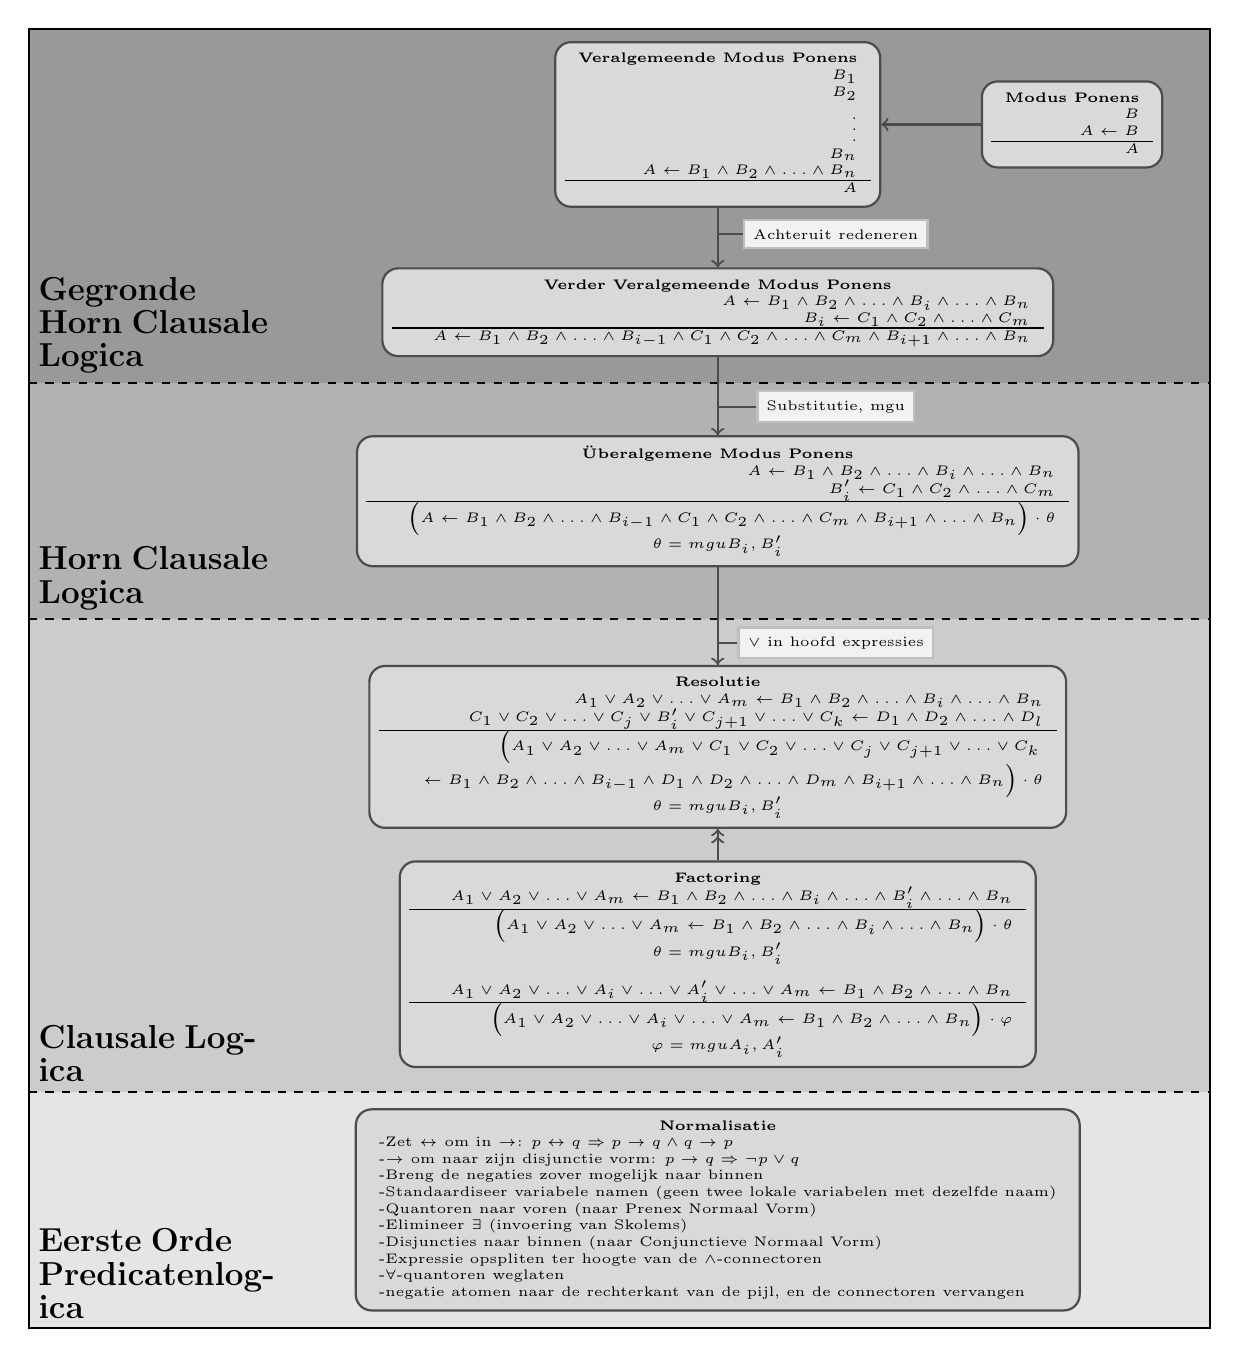
\begin{tikzpicture}[taal/.style={anchor=south west,text width=90pt},taalT/.style={draw=green,thick,fill=green!50},taalF/.style={draw=black!70,thick,fill=blue!50,rounded corners=2mm},concept/.style={draw=black!70,thick,fill=black!15,rounded corners=2mm},conceptgeneral/.style={thick,->,black!70},principle/.style={draw=black!25,thick,fill=black!5},principleused/.style={black!70,thick}]
\def\rectW{15};
\def\trapa{4.5};
\def\trapb{7.5};
\def\trapc{13.5};
\def\trapd{16.5};
\def\rectH{16.5};
\def\column{-0.5*\rectW+3.25};
\def\barW{\rectW-3.25};
\def\colF{4};
\def\xT{\column+2+0.3*\barW};
\def\xF{\column+2+0.5*\barW};
\def\xCa{\column+2+0.45*\barW};
\def\xCb{\column+2+0.55*\barW};
\def\xCc{\column+2+0.75*\barW};

\fill[black!40] (-0.5*\rectW,0) rectangle (0.5*\rectW,-\trapa);
\fill[black!30] (-0.5*\rectW,-\trapa) rectangle (0.5*\rectW,-\trapb);
\fill[black!20] (-0.5*\rectW,-\trapb) rectangle (0.5*\rectW,-\trapc);
\fill[black!10] (-0.5*\rectW,-\trapc) rectangle (0.5*\rectW,-\trapd);
\draw[thick] (-0.5*\rectW,0) rectangle (0.5*\rectW,-\rectH);
\draw[thick,dashed] (-0.5*\rectW,-\trapa) -- (0.5*\rectW,-\trapa);
\draw[thick,dashed] (-0.5*\rectW,-\trapb) -- (0.5*\rectW,-\trapb);
\draw[thick,dashed] (-0.5*\rectW,-\trapc) -- (0.5*\rectW,-\trapc);

\node[taal] (trapaL) at (-0.5*\rectW,-\trapa) {\bf \large Gegronde Horn Clausale Logica};
\node[concept] (trapaC1) at (\xCc,-0.27*\trapa) {\tiny$\begin{array}{lr}\multicolumn{2}{c}{\mbox{\bf Modus Ponens}}\\&B\\\therefore&A\leftarrow B\\\hline&A\end{array}$};
\node[concept] (trapaC2) at (\xCa,-0.27*\trapa) {\tiny$\begin{array}{lr}\multicolumn{2}{c}{\mbox{\bf Veralgemeende Modus Ponens}}\\&B_1\\&B_2\\&\vdots\\&B_n\\\therefore&A\leftarrow B_1\wedge B_2\wedge\ldots\wedge B_n\\\hline&A\end{array}$};
\node[concept] (trapaC3) at (\xCa,-0.8*\trapa) {\tiny$\begin{array}{lr}\multicolumn{2}{c}{\mbox{\bf Verder Veralgemeende Modus Ponens}}\\&A\leftarrow B_1\wedge B_2\wedge\ldots\wedge B_i\wedge\ldots\wedge B_n\\\therefore&B_i\leftarrow C_1\wedge C_2\wedge\ldots\wedge C_m\\\hline&A\leftarrow B_1\wedge B_2\wedge\ldots\wedge B_{i-1}\wedge C_1\wedge C_2\wedge\ldots\wedge C_m\wedge B_{i+1}\wedge\ldots\wedge B_n\end{array}$};
\node[principle] (trapaP1) at (\xCb,-0.58*\trapa) {\tiny Achteruit redeneren};
\draw[principleused] (trapaC3.north) |- (trapaP1.west);
\draw[conceptgeneral] (trapaC1) -- (trapaC2);
\draw[conceptgeneral] (trapaC2) -- (trapaC3);

\node[taal] (trapbL) at (-0.5*\rectW,-\trapb) {\bf \large Horn Clausale Logica};
\node[concept] (trapbC1) at (\xCa,-0.5*\trapa-0.5*\trapb) {\tiny$\begin{array}{lr}\multicolumn{2}{c}{\mbox{\bf \"Uberalgemene Modus Ponens}}\\&A\leftarrow B_1\wedge B_2\wedge\ldots\wedge B_i\wedge\ldots\wedge B_n\\\therefore&B_i'\leftarrow C_1\wedge C_2\wedge\ldots\wedge C_m\\\hline&\left(A\leftarrow B_1\wedge B_2\wedge\ldots\wedge B_{i-1}\wedge C_1\wedge C_2\wedge\ldots\wedge C_m\wedge B_{i+1}\wedge\ldots\wedge B_n\right)\cdot\theta\\\multicolumn{2}{c}{\theta=\mathfunc{mgu}{B_i,B_i'}}\end{array}$};
\node[principle] (trapbP1) at (\xCb,-0.9*\trapa-0.1*\trapb) {\tiny Substitutie, mgu};
\draw[principleused] (trapbC1.north) |- (trapbP1.west);
\draw[conceptgeneral] (trapaC3) -- (trapbC1);

\node[taal] (trapcL) at (-0.5*\rectW,-\trapc) {\bf \large Clausale Logica};
\node[concept] (trapcC1) at (\xCa,-0.27*\trapc-0.73*\trapb) {\tiny$\begin{array}{lr}\multicolumn{2}{c}{\mbox{\bf Resolutie}}\\
&A_1\vee A_2\vee\ldots\vee A_m\leftarrow B_1\wedge B_2\wedge\ldots\wedge B_i\wedge\ldots\wedge B_n\\\therefore&C_1\vee C_2\vee\ldots\vee C_j\vee B_i'\vee C_{j+1}\vee\ldots\vee C_k\leftarrow D_1\wedge D_2\wedge\ldots\wedge D_l\\\hline&\left(A_1\vee A_2\vee\ldots\vee A_m\vee C_1\vee C_2\vee\ldots\vee C_j\vee C_{j+1}\vee\ldots\vee C_k\right.\\&\left.\leftarrow B_1\wedge B_2\wedge\ldots\wedge B_{i-1}\wedge D_1\wedge D_2\wedge\ldots\wedge D_m\wedge B_{i+1}\wedge\ldots\wedge B_n\right)\cdot\theta\\\multicolumn{2}{c}{\theta=\mathfunc{mgu}{B_i,B_i'}}\end{array}$};
\node[concept] (trapcC2) at (\xCa,-0.73*\trapc-0.27*\trapb) {\tiny$\begin{array}{lr}\multicolumn{2}{c}{\mbox{\bf Factoring}}\\\therefore&A_1\vee A_2\vee\ldots\vee A_m\leftarrow B_1\wedge B_2\wedge\ldots\wedge B_i\wedge\ldots\wedge B_i'\wedge\ldots\wedge B_n\\\hline&\left(A_1\vee A_2\vee\ldots\vee A_m\leftarrow B_1\wedge B_2\wedge\ldots\wedge B_i\wedge\ldots\wedge B_n\right)\cdot\theta\\\multicolumn{2}{c}{\theta=\mathfunc{mgu}{B_i,B_i'}}\\\\
\therefore&A_1\vee A_2\vee\ldots\vee A_i\vee\ldots\vee A_i'\vee\ldots\vee A_m\leftarrow B_1\wedge B_2\wedge\ldots\wedge B_n\\\hline&\left(A_1\vee A_2\vee\ldots\vee A_i\vee\ldots\vee A_m\leftarrow B_1\wedge B_2\wedge\ldots\wedge B_n\right)\cdot\varphi\\\multicolumn{2}{c}{\varphi=\mathfunc{mgu}{A_i,A_i'}}\end{array}$};
\node[principle] (trapcP1) at (\xCb,-0.95*\trapb-0.05*\trapc) {\tiny $\vee$ in hoofd expressies};
\draw[principleused] (trapcC1.north) |- (trapcP1.west);
\draw[conceptgeneral] (trapbC1) -- (trapcC1);
\draw[conceptgeneral,<<-] (trapcC1) -- (trapcC2);

\node[taal] (trapdL) at (-0.5*\rectW,-\trapd) {\bf \large Eerste Orde Predicatenlogica};
\node[concept] (trapaL) at (\xCa,-0.5*\trapd-0.5*\trapc) {\tiny$\begin{array}{l}\multicolumn{1}{c}{\mbox{\bf Normalisatie}}\\\mbox{-Zet $\leftrightarrow$ om in $\rightarrow$: $p\leftrightarrow q\Rightarrow p\rightarrow q\wedge q\rightarrow p$}\\\mbox{-$\rightarrow$ om naar zijn disjunctie vorm: $p\rightarrow q\Rightarrow \neg p\vee q$}\\\mbox{-Breng de negaties zover mogelijk naar binnen}\\\mbox{-Standaardiseer variabele namen (geen twee lokale variabelen met dezelfde naam)}\\\mbox{-Quantoren naar voren (naar Prenex Normaal Vorm)}\\\mbox{-Elimineer $\exists$ (invoering van Skolems)}\\\mbox{-Disjuncties naar binnen (naar Conjunctieve Normaal Vorm)}\\\mbox{-Expressie opspliten ter hoogte van de $\wedge$-connectoren}\\\mbox{-$\forall$-quantoren weglaten}\\\mbox{-negatie atomen naar de rechterkant van de pijl, en de connectoren vervangen}\end{array}$};
\end{tikzpicture}
\caption{Samenvattend schema van Automatisch Redeneren}
\end{figure}
\subsection{Metaheuristieken}
\begin{figure}[H]
\centering
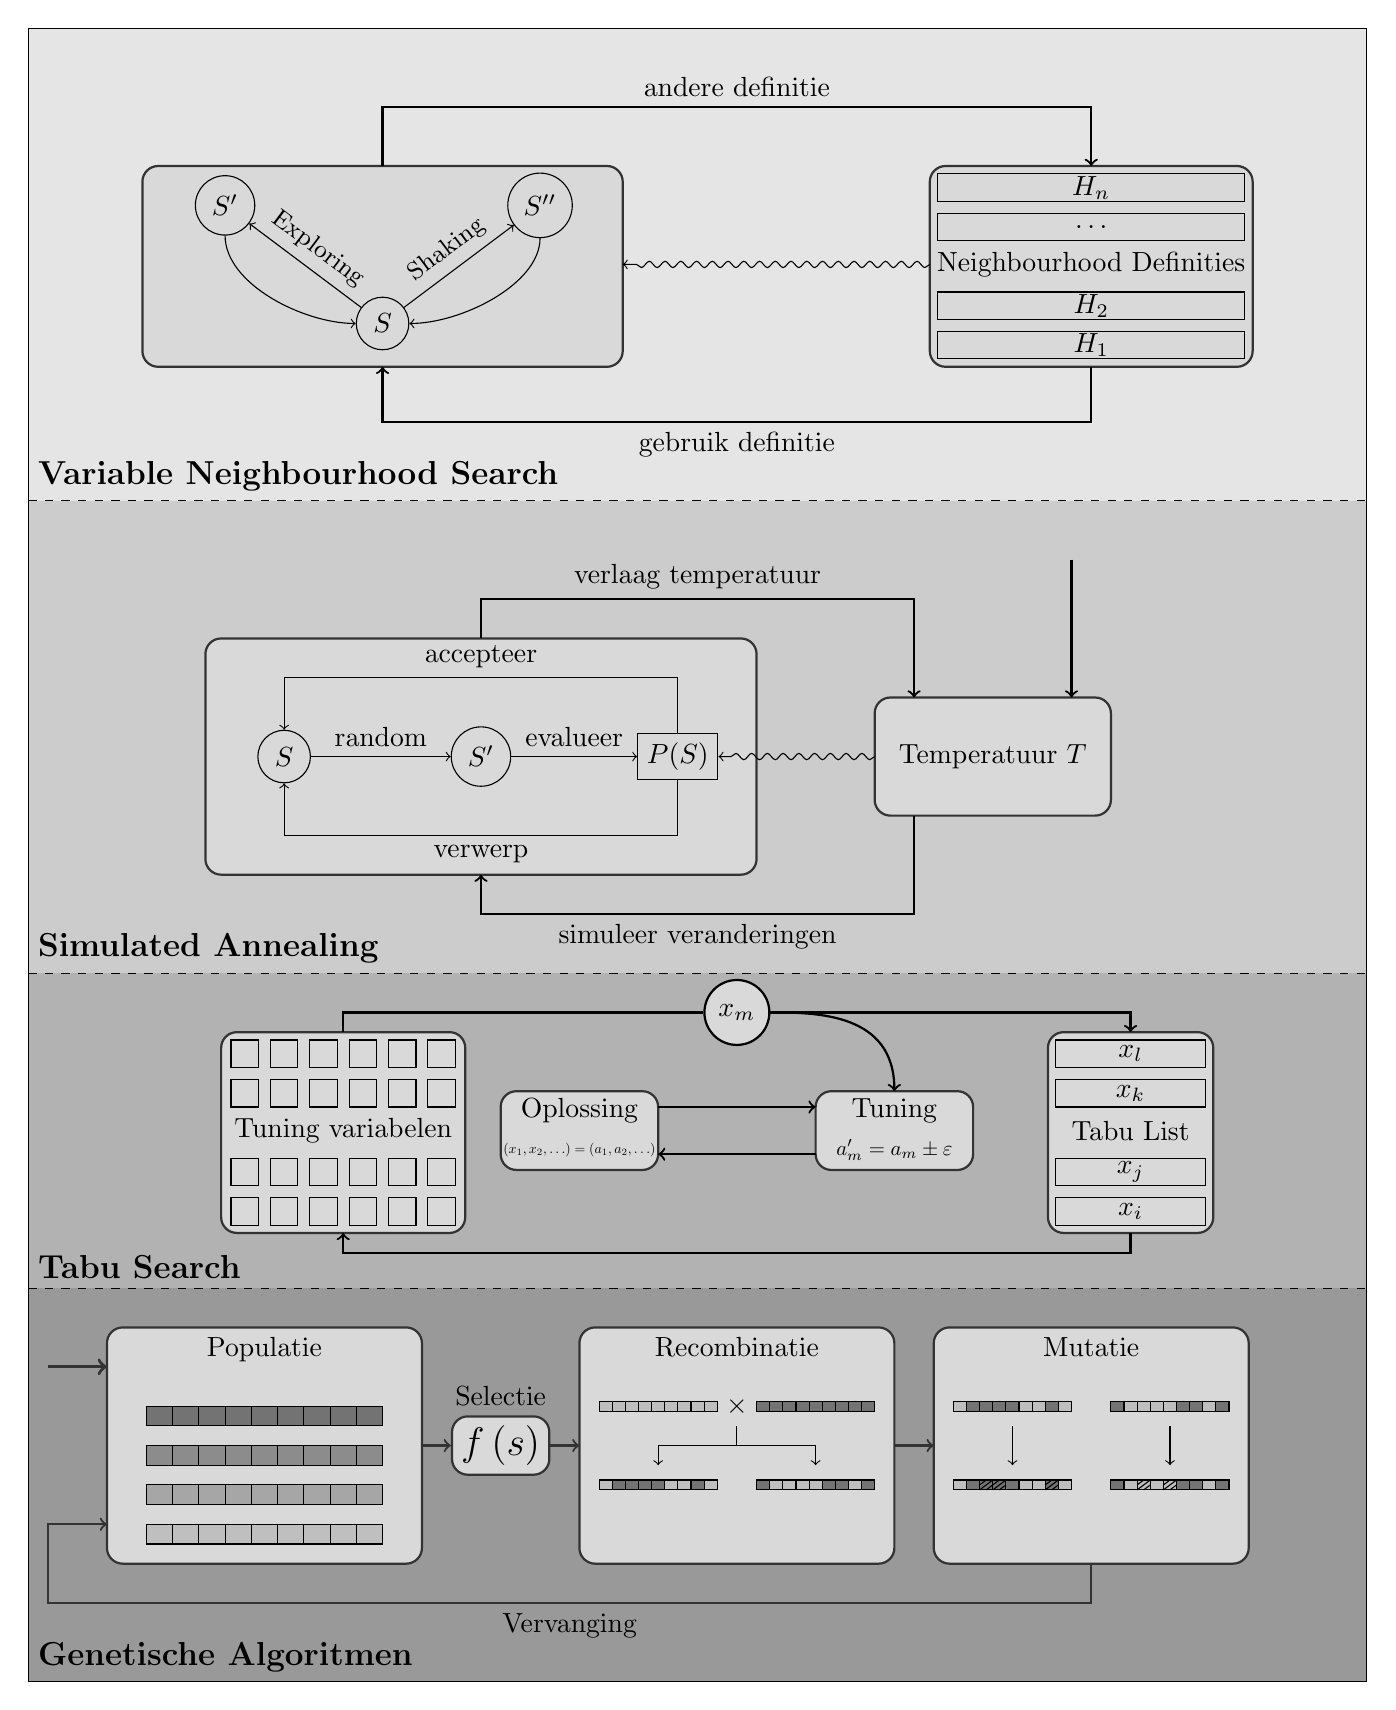
\begin{tikzpicture}[concclass/.style={anchor=south west},conceptgroup/.style={draw=black!80, thick,fill=black!15, rounded corners=2mm},conceptname/.style={anchor=north},cname/.style={conceptgroup},conceptarr/.style={black!80,thick,->}]
\fill[black!40] (-2,-0.5) rectangle (15,4.5);
\fill[black!30] (-2,4.5) rectangle (15,8.5);
\fill[black!20] (-2,8.5) rectangle (15,14.5);
\fill[black!10] (-2,14.5) rectangle (15,20.5);
\draw (-2,-0.5) rectangle (15,20.5);
\draw[dashed] (-2,4.5) -- (15,4.5);
\draw[dashed] (-2,8.5) -- (15,8.5);
\draw[dashed] (-2,14.5) -- (15,14.5);

\draw[concclass] (-2,-0.5) node{\bf \large Genetische Algoritmen};
\draw[conceptgroup] (-1,4) rectangle (3,1);
\node[conceptname] (Pop) at (1,4) {Populatie};
\foreach\y/\c in {1/25,2/35,3/45,4/55} {
  \fill[black!\c] (-0.5,0.5*\y+0.75) rectangle (2.5,0.5*\y+1);
  \draw[black] (-0.5,0.5*\y+0.75) rectangle (2.5,0.5*\y+1);
  \foreach \x in {1,2,...,8} {
    \draw[black] (-0.5+\x/3,0.5*\y+0.75) -- (-0.5+\x/3,0.5*\y+1);
  }
}
\draw[conceptarr,very thick] (-1.75,3.5) -- (-1,3.5);
\node[cname] (Eva) at (4,2.5) {\Large $f\left(s\right)$};
\node[conceptname,anchor=south] (Sel) at (Eva.north) {Selectie};
\draw[conceptarr] (3,2.5) -- (Eva);
\draw[conceptgroup] (5,4) rectangle (9,1);
\node[conceptname] (Pop) at (7,4) {Recombinatie};
\draw (7,3) node {$\times$};
\fill[black!25,draw=black] (5.25,2.9375) rectangle (6.75,3.0625);
\fill[black!55,draw=black] (7.25,2.9375) rectangle (8.75,3.0625);
\fill[black!25] (5.25,1.9375) rectangle (6.75,2.0625);
\fill[black!55] (7.25,1.9375) rectangle (8.75,2.0625);
\foreach \x/\y in {1/5,7/8} {
  \fill[black!55] (5.25+\x/6,1.9375) rectangle (5.25+\y/6,2.0625);
  \fill[black!25] (7.25+\x/6,1.9375) rectangle (7.25+\y/6,2.0625);
}
\draw (5.25,1.9375) rectangle (6.75,2.0625);
\draw (7.25,1.9375) rectangle (8.75,2.0625);
\draw (7,2.75) -- (7,2.5);
\draw[<->] (6,2.25) -- (6,2.5) -- (8,2.5) -- (8,2.25);
\foreach \x in {1,2,...,8} {
  \draw[black] (5.25+\x/6,2.9375) -- (5.25+\x/6,3.0625);
  \draw[black] (7.25+\x/6,2.9375) -- (7.25+\x/6,3.0625);
  \draw[black] (5.25+\x/6,1.9375) -- (5.25+\x/6,2.0625);
  \draw[black] (7.25+\x/6,1.9375) -- (7.25+\x/6,2.0625);
}
\draw[conceptarr] (Eva) -- (5,2.5);
\draw[conceptgroup] (9.5,4) rectangle (13.5,1);
\node[conceptname] (Pop) at (11.5,4) {Mutatie};
\fill[black!25] (9.75,2.9375) rectangle (11.25,3.0625);
\fill[black!55] (11.75,2.9375) rectangle (13.25,3.0625);
\fill[black!25] (9.75,1.9375) rectangle (11.25,2.0625);
\fill[black!55] (11.75,1.9375) rectangle (13.25,2.0625);
\foreach \x/\y in {1/5,7/8} {
  \fill[black!55] (9.75+\x/6,2.9375) rectangle (9.75+\y/6,3.0625);
  \fill[black!25] (11.75+\x/6,2.9375) rectangle (11.75+\y/6,3.0625);
  \fill[black!55] (9.75+\x/6,1.9375) rectangle (9.75+\y/6,2.0625);
  \fill[black!25] (11.75+\x/6,1.9375) rectangle (11.75+\y/6,2.0625);
}
\foreach \x in {2,3,7} {
  \draw (9.75+\x/6,1.9375) -- (9.75+\x/6+1/6,2.0625);
  \draw (9.75+1/12+\x/6,1.9375) -- (9.75+\x/6+1/6,2);
  \draw (9.75+\x/6,2) -- (9.75+\x/6+1/12,2.0625);
}
\foreach \x in {2,4} {
  \draw (11.75+\x/6,1.9375) -- (11.75+\x/6+1/6,2.0625);
  \draw (11.75+1/12+\x/6,1.9375) -- (11.75+\x/6+1/6,2);
  \draw (11.75+\x/6,2) -- (11.75+\x/6+1/12,2.0625);
}
\draw[->] (10.5,2.75) -- (10.5,2.25);
\draw[->] (12.5,2.75) -- (12.5,2.25);
\draw (9.75,2.9375) rectangle (11.25,3.0625);
\draw (11.75,2.9375) rectangle (13.25,3.0625);
\draw (9.75,1.9375) rectangle (11.25,2.0625);
\draw (11.75,1.9375) rectangle (13.25,2.0625);
\foreach \x in {1,2,...,8} {
  \draw[black] (9.75+\x/6,2.9375) -- (9.75+\x/6,3.0625);
  \draw[black] (11.75+\x/6,2.9375) -- (11.75+\x/6,3.0625);
  \draw[black] (9.75+\x/6,1.9375) -- (9.75+\x/6,2.0625);
  \draw[black] (11.75+\x/6,1.9375) -- (11.75+\x/6,2.0625);
}
\draw[conceptarr] (9,2.5) -- (9.5,2.5);
\draw[conceptarr] (11.5,1) -- (11.5,0.5) to node[black,midway,below]{Vervanging} (-1.75,0.5) -- (-1.75,1.5) -- (-1,1.5);

\draw[concclass] (-2,4.5) node{\bf \large Tabu Search};
\draw[concclass] (-2,8.5) node{\bf \large Simulated Annealing};
\draw[concclass] (-2,14.5) node{\bf \large Variable Neighbourhood Search};
\begin{scope}[xshift=12 cm,yshift=6.5 cm]
\draw[conceptgroup] (-1.05,-1.3) rectangle (1.05,1.25);
\draw (0,0) node {Tabu List};
\foreach\y/\t in {1/i,2/j,4/k,5/l} {
  \draw (-0.95,-1.7+0.5*\y) rectangle (0.95,-1.35+0.5*\y);
  \draw (0,-1.525+0.5*\y) node{$x_\t$};
}
\draw[conceptgroup] (-11.55,-1.3) rectangle (-8.45,1.25);
\draw (-10,0) node {Tuning variabelen};
\foreach\y in {1,2,4,5} {
  \foreach\x in {0,1,2,3,4,5} {
    \draw (-11.425+0.5*\x,-1.7+0.5*\y) rectangle ++(0.35,0.35);
  }
}
\draw[conceptgroup] (-8,-0.5) rectangle (-6,0.5);
\draw (-7,0.25) node {Oplossing};
\draw (-7,-0.25) node[scale=0.5] {$\left(x_1,x_2,\ldots\right)=\left(a_1,a_2,\ldots\right)$};
\draw[conceptgroup] (-4,-0.5) rectangle (-2,0.5);
\draw (-3,-0.25) node[scale=0.75] {$a_m'=a_m\pm\varepsilon$};
\draw (-3,0.25) node {Tuning};
\node[conceptgroup,draw=black,circle,thick] (V) at (-5,1.5) {$x_m$};
\draw[thick,->] (-10,1.25) |- (V) -| (0,1.25);
\draw[thick,->] (0,-1.3) |- (-5,-1.55) -| (-10,-1.3);
\draw[thick,->] (-6,0.3) -- (-4,0.3);
\draw[thick,->] (-4,-0.3) -- (-6,-0.3);
\draw[thick,->] (V) .. controls ++(1,0) and (-3,1.5) .. (-3,0.5);
\end{scope}
\begin{scope}[xshift=3.75 cm,yshift=11.25 cm]
\draw[conceptgroup] (5,-0.75) rectangle (8,0.75);
\draw (6.5,0) node {Temperatuur $T$};
\draw[conceptgroup] (-3.5,-1.5) rectangle (3.5,1.5);
\node[draw=black,circle] (S1) at (-2.5,0) {$S$};
\node[draw=black,circle] (S2) at (0,0) {$S'$};
\node[draw=black,rectangle] (P) at (2.5,0) {$P(S)$};
\draw[->] (S1) to node[midway,sloped,above]{random} (S2);
\draw[->] (S2) to node[midway,sloped,above]{evalueer} (P);
\draw[->] (P.south) -- (2.5,-1) to node[below,midway,sloped] {verwerp} (-2.5,-1) -- (S1);
\draw[->] (P.north) -- (2.5,1) to node[above,midway,sloped] {accepteer} (-2.5,1) -- (S1);
\draw[->,decorate,decoration={snake,amplitude=.4mm,segment length=2mm,post length=1mm}] (5,0) -- (P);
\draw[thick,->] (7.5,2.5) -- (7.5,0.75);
\draw[thick,->] (0,1.5) -- (0,2) to node[midway,sloped,above]{verlaag temperatuur} (5.5,2) -- (5.5,0.75);
\draw[thick,->] (5.5,-0.75) -- (5.5,-2) to node[midway,sloped,below]{simuleer veranderingen} (0,-2) -- (0,-1.5);
\end{scope}
\begin{scope}[xshift=11.5 cm,yshift=17.5 cm]
\draw[conceptgroup] (-2.05,-1.3) rectangle (2.05,1.25);
\draw (0,0) node {Neighbourhood Definities};
\foreach\y/\t in {1/\mathfrak{H}_1,2/\mathfrak{H}_2,4/\ldots,5/\mathfrak{H}_n} {
  \draw (-1.95,-1.7+0.5*\y) rectangle (1.95,-1.35+0.5*\y);
  \draw (0,-1.525+0.5*\y) node{$\t$};
}
\draw[conceptgroup] (-12.05,-1.3) rectangle (-5.95,1.25);
\node[draw=black,circle] (S) at (-9,-0.75) {$S$};
\node[draw=black,circle] (S1) at (-11,0.75) {$S'$};
\node[draw=black,circle] (S2) at (-7,0.75) {$S''$};
\draw[->] (S) to node[sloped,midway,above]{\small{Exploring}} (S1);
\draw[->] (S) to node[sloped,midway,above]{\small{Shaking}} (S2);
\draw[->] (S1) .. controls ++(0,-1) and (-10,-0.75) .. (S);
\draw[->] (S2) .. controls ++(0,-1) and (-8,-0.75) .. (S);
\draw[->,decorate,decoration={snake,amplitude=.4mm,segment length=2mm,post length=1mm}] (-2.05,0) -- (-5.95,0);
\draw[->,thick] (0,-1.3) -- (0,-2) to node[midway,sloped,below]{gebruik definitie} (-9,-2) -- (-9,-1.3);
\draw[->,thick] (-9,1.25) -- (-9,2) to node[midway,sloped,above]{andere definitie} (0,2) -- (0,1.25);
\end{scope}
\end{tikzpicture}
\caption{Samenvattend schema van Metaheuristieken}
\end{figure}
